\documentclass[]{article}
\usepackage{amsmath}
\usepackage{graphicx}
\usepackage{listings}
\usepackage{color}

\definecolor{dkgreen}{rgb}{0,0.6,0}
\definecolor{gray}{rgb}{0.5,0.5,0.5}
\definecolor{mauve}{rgb}{0.58,0,0.82}

\lstset{frame=tb,
	language=R,
	aboveskip=3mm,
	belowskip=3mm,
	showstringspaces=false,
	columns=flexible,
	basicstyle={\small\ttfamily},
	numbers=none,
	numberstyle=\tiny\color{gray},
	keywordstyle=\color{blue},
	commentstyle=\color{dkgreen},
	stringstyle=\color{mauve},
	breaklines=true,
	breakatwhitespace=true,
	tabsize=3
}

\title{A Template}
\begin{document}
	
\section{Conway-Maxwell Poisson (COM-Poisson, CMP) and Properties}
The p.m.f. for Conway-Maxwell Poisson (CMP) is:
\begin{equation*}
	P(Y = y|\lambda, \nu) = \frac{\lambda^{y}}{(y!)^{\nu}}\frac{1}{Z(\lambda, \nu)}
\end{equation*}
$Z(\lambda, \nu) = Z$ is the normalization constant, i.e. $Z(\lambda, \nu) = Z = \sum_{y=0}^{\infty}\frac{\lambda^{y}}{(y!)^{\nu}}$, which doesn't have closed form in general. The domain for parameters is $\lambda, \nu > 0$ and $0 < \lambda < 1, \nu = 0$. The parameter $\nu$ controls the dispersion: 1) when $\nu = 1$, the CMP is Poisson distribution, 2) when $\nu < 1$, the distribution is over-dispersed and 3) when $\nu > 1$, the distribution is under-dispersed. When $\nu\to\infty$, the CMP approaches a Bernoulli distribution, while $\nu=0$, it reduces to a geometric distribution.\\
\\
To model the mean and dispersion simultaneously, two linear models are used for parameters $\lambda$ and $\nu$, i.e. $\log(\lambda) = \boldsymbol{x}'\boldsymbol{\beta}$ and $\log(\nu) = \boldsymbol{g}'\boldsymbol{\gamma}$, in this manuscript, I further define $\boldsymbol{\theta}' = (\boldsymbol{\beta}', \boldsymbol{\gamma}')$.\\
\\
To derive the SSP for CMP regression, the keys are gradient and Hessian for log-likelihood. In the following part of this section, I will define some notations and give some necessary properties for CMP.\\
\\
Assume there are n independent $Y_i \sim CMP(\lambda_i, \nu_i)$. Denote $\boldsymbol{\eta}_i = (log(\lambda_i), \nu_i)'$, $Z_i = Z(\lambda_i, \nu_i)$ The log-likelihood for $i^{th}$ observation is:
\begin{align*}
	l_i(\boldsymbol{\eta}_i) &=  y_i log(\lambda_i) - log(y_i!)\nu_i - log(Z_i)
\end{align*}
Since $E(Y_i) = \frac{\partial log(Z_i)}{\partial log(\lambda_i)}$, $Var(Y_i) = \frac{\partial^2 log(Z_i)}{\partial log(\lambda_i)^2}$, $E(log(Y_i!)) = -\frac{\partial log(Z_i)}{\partial \nu_i}$, $Var(log(Y_i!)) = \frac{\partial^2 log(Z_i)}{\partial \nu_i^2}$ and $Cov(Y_i, log(Y_i!)) = -\frac{\partial^2log(Z_i)}{\partial log(\lambda_i) \partial \nu_i}$, the gradient for $l_i$ (w.r.t $\boldsymbol{\eta}_i$) is:
\begin{equation*}
	\frac{\partial l_i}{\partial \boldsymbol{\eta}_i} = 
	\begin{pmatrix} y_i - E(Y_i)\\
		E(log(Y_i!)) - log(y_i!)
	\end{pmatrix}
\end{equation*}
And the Hessian for $l_i$ (w.r.t $\boldsymbol{\eta}_i$) is:
\begin{equation*}
	\frac{\partial^2 l_i}{\partial \boldsymbol{\eta_i}\partial \boldsymbol{\eta_i}'}= 
	\begin{pmatrix} -Var(Y_i) & Cov(Y_i, log(Y_i!))\\
		Cov(Y_i, log(Y_i!)) & -Var(log(Y_i!))
	\end{pmatrix}
\end{equation*}

The moments $E(Y_i)$, $Var(Y_i)$, $E(log(Y_i!))$, $Var(log(Y_i!))$ and $Cov(Y_i, log(Y_i!))$ by using the following approximation for normalizing constant $Z_i$:
\begin{equation*}
	Z_i = \frac{e^{\nu_i \lambda_i^{1/\nu_i}}}{\lambda_i^{\frac{\nu_i-1}{2\nu_i}}}\left(1 + c_1(\nu_i \lambda_i^{1/\nu_i})^{-1} + c_2(\nu_i \lambda_i^{1/nu_i})^{-2} + \mathcal{O}(\lambda_i^{\frac{-3}{\nu_i}})\right)
\end{equation*}
\\
The approximation works well when $\lambda_i \geq 2$ and $\nu_i \leq 1$, and this can be helpful when updating/ calculating the gradient and hessian matrix. Currently, I didn't use this approximation for simplicity.\\
\\
If we use models $\log(\lambda_i) = \boldsymbol{x_i}'\boldsymbol{\beta}$ and $\log(\nu_i) = \boldsymbol{g_i}'\boldsymbol{\gamma}$, by using chain rule, the gradient for $l_i$ (w.r.t $\boldsymbol{\theta}$) is:
\begin{equation*}
	\frac{\partial l_i}{\partial \boldsymbol{\theta}} = 
	 = \begin{pmatrix} [y_i - E(Y_i)]\boldsymbol{x_i}\\
		\nu_i[E(log(Y_i!)) - log(y_i!)]\boldsymbol{g_i}
	\end{pmatrix}
\end{equation*}
And the Hessian for $l_i$ (w.r.t $\boldsymbol{\theta}$) is:
\begin{equation*}
	\frac{\partial^2 l_i}{\partial \boldsymbol{\theta}\partial \boldsymbol{\theta}'} = 
	\begin{pmatrix} -Var(Y_i)\boldsymbol{x_i}\boldsymbol{x_i}' &
		 \nu_i Cov(Y_i, log(Y_i!))\boldsymbol{x_i}\boldsymbol{g_i}'\\
		\nu_i Cov(Y_i, log(Y_i!))\boldsymbol{g_i}\boldsymbol{x_i}' &
		 -\nu_i[\nu_i Var(log(Y_i!) - E(log(Y_i!)) + log(y_i!))]\boldsymbol{g_i}\boldsymbol{g_i}'
	\end{pmatrix}
\end{equation*}

\section{SSP for CMP}
By denoting $a_i = [y_i - E(Y_i| \hat{\boldsymbol{\theta}}_{MLE})]$ and $b_i = 	\nu_i(\hat{\boldsymbol{\theta}}_{MLE})[E(log(Y_i!)| \hat{\boldsymbol{\theta}}_{MLE}) - log(y_i!)]$, we define 
$$\boldsymbol{V}_c = \frac{1}{rn^2}\sum_{i=1}^{n}\frac{1}{\pi_i}\begin{pmatrix}
	a_i^2\boldsymbol{x_i}\boldsymbol{x_i}' &
	a_i b_i\boldsymbol{x_i}\boldsymbol{g_i}'\\
	a_i b_i\boldsymbol{g_i}\boldsymbol{x_i}' &
	b_i^2\boldsymbol{g_i}\boldsymbol{g_i}'
\end{pmatrix}$$
where $r$ is the subsample size, with subsampling probabilities $\pi_i$ for all data points.\\
\\
Further we denote the observed information matrix as
$$
\boldsymbol{M}_X = \frac{1}{n}\sum_{i=1}^{n}\begin{pmatrix}
	A_i & B_i\\
	B_i^{'} & C_i
\end{pmatrix}
$$
where
\begin{align*}
	A_i &= Var(Y_i|\hat{\boldsymbol{\theta}}_{MLE})\boldsymbol{x_i}\boldsymbol{x_i}'\\
	B_i &= -\nu_i(\hat{\boldsymbol{\theta}}_{MLE}) Cov(Y_i, log(Y_i!)| \hat{\boldsymbol{\theta}}_{MLE})\boldsymbol{x_i}\boldsymbol{g_i}'\\
	C_i &= \nu_i(\hat{\boldsymbol{\theta}}_{MLE})[\nu_i(\hat{\boldsymbol{\theta}}_{MLE}) Var(log(Y_i!|\hat{\boldsymbol{\theta}}_{MLE}) - E(log(Y_i!|\hat{\boldsymbol{\theta}}_{MLE})) + log(y_i!))]\boldsymbol{g_i}\boldsymbol{g_i}'
\end{align*}

Then follow the same steps as in OSMAC, we can show that as $n \to \infty$ and $r \to \infty$, conditional on full data matrix $\mathcal{F}_n = \boldsymbol{X}, \boldsymbol{y}$ in probability,
$$
\boldsymbol{V}^{-1/2}(\tilde{\boldsymbol{\theta}} - \hat{\boldsymbol{\theta}}_{MLE}) \to N(0, \boldsymbol{I})
$$
where $\boldsymbol{V} = \boldsymbol{M}_X^{-1}\boldsymbol{V}_c\boldsymbol{M}_X^{-1}$ and $\tilde{\boldsymbol{\theta}}$ is the sub-sampling estimates for $\boldsymbol{\theta}$
\\
Then under A-optimality criterion, the sub-sampling probabilities (SSPs) $\pi_i^{mMSE}$ are proportional to $||\boldsymbol{M}_X^{-1}\begin{pmatrix}
	a_i\boldsymbol{x}_i\\b_i\boldsymbol{g}_i
\end{pmatrix}||$, while under L-optimality criterion, $\pi_i^{mVc} \propto ||\begin{pmatrix}
a_i\boldsymbol{x}_i\\b_i\boldsymbol{g}_i
\end{pmatrix}||$. In other words:
\begin{align*}
	\pi_i^{mMSE} &= \frac{||\boldsymbol{M}_X^{-1}\begin{pmatrix}
			[y_i - E(Y_i| \hat{\boldsymbol{\theta}}_{MLE})]\boldsymbol{x}_i\\
			\nu_i(\hat{\boldsymbol{\theta}}_{MLE})[E(log(Y_i!)| \hat{\boldsymbol{\theta}}_{MLE}) - log(y_i!)]\boldsymbol{g}_i
		\end{pmatrix}||}{\sum_{j=1}^{n}||\boldsymbol{M}_X^{-1}\begin{pmatrix}
			[y_j - E(Y_j| \hat{\boldsymbol{\theta}}_{MLE})]\boldsymbol{x}_j\\
			\nu_j(\hat{\boldsymbol{\theta}}_{MLE})[E(log(Y_j!)| \hat{\boldsymbol{\theta}}_{MLE}) - log(y_j!)]\boldsymbol{g}_j
		\end{pmatrix}||}\\
	\pi_i^{mVc} &= \frac{||\begin{pmatrix}
			[y_i - E(Y_i| \hat{\boldsymbol{\theta}}_{MLE})]\boldsymbol{x}_i\\
			\nu_i(\hat{\boldsymbol{\theta}}_{MLE})[E(log(Y_i!)| \hat{\boldsymbol{\theta}}_{MLE}) - log(y_i!)]\boldsymbol{g}_i
		\end{pmatrix}||}{\sum_{j=1}^{n}||\begin{pmatrix}
			[y_j - E(Y_j| \hat{\boldsymbol{\theta}}_{MLE})]\boldsymbol{x}_j\\
			\nu_j(\hat{\boldsymbol{\theta}}_{MLE})[E(log(Y_j!)| \hat{\boldsymbol{\theta}}_{MLE}) - log(y_j!)]\boldsymbol{g}_j
		\end{pmatrix}||}
\end{align*}

\section{Necessity for fitting CMP model}
Here I first generate the data by CMP distribution.\\
\\
There are $n = 10000$ independent observations, with $Y_i \sim CMP(\lambda_i, \nu_i)$ for $i = 1, 2,..., n$. The $\lambda_i$ and $\nu_i$ are modeled as:
\begin{align*}
	\lambda_i &= \exp(x_{i1})\\
	\nu_i &= \exp(1 + g_{i1})
\end{align*}
where $x_{i1} \stackrel{i.i.d.}{\sim} N(0, 1)$ and $g_{i1} \stackrel{i.i.d.}{\sim} N(1, 1)$ The following two plots show the fitted mean and median for 1) Poisson regression, 2) CMP regression, with constant $\nu_i = \nu$ (constant CMP) and 3) CMP with $\nu_i$ modeled by $g_{i1}$ (full CMP).\\
\graphicspath{{D:/GitHub/sub-sampling/COM-Poisson/cdoe/}}
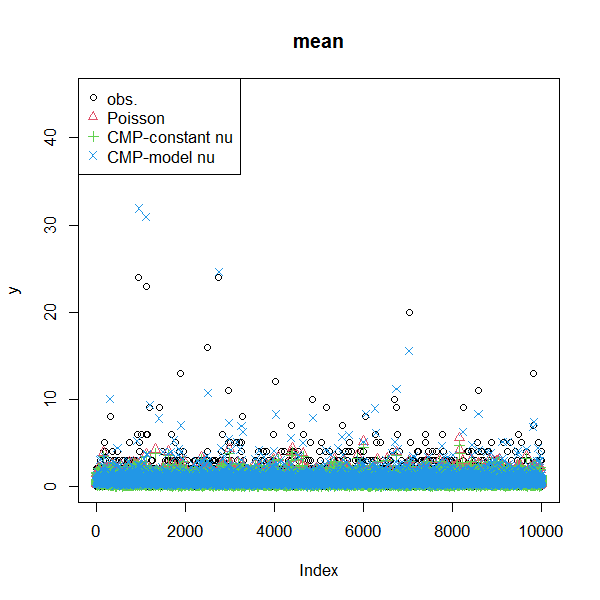
\includegraphics[width = .6\textwidth]{mean.png}
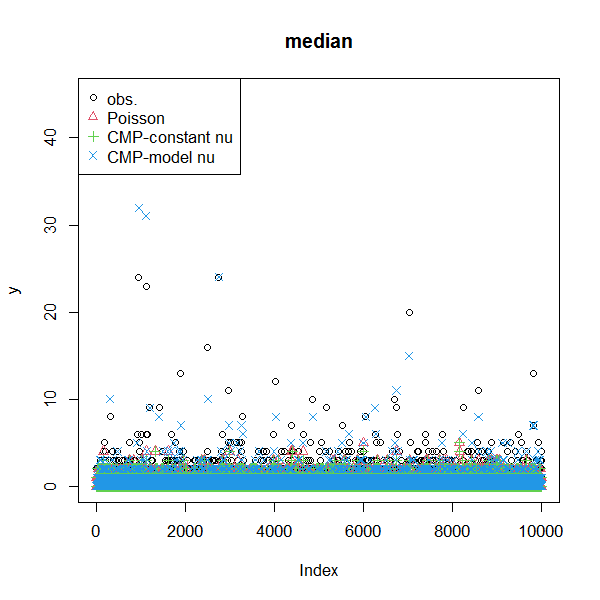
\includegraphics[width = .6\textwidth]{median.png}
The MSEs ($\frac{(Y_i - \hat{Y})^2}{n}$) for mean are 1) Poisson: 2.269, 2) constant CMP: 2.273 and 3) full CMP: 0.391. The Poisson model and constant dispersion CMP model are not good for handling extreme observations. Therefore, it's necessary to take dispersion into account and CMP is a good choice.\\
\\
The running time for these three: 1)Poisson: 0.03s, 2) constant CMP: 2.40s and 3) full CMP: 3.59s. This shows that CMP regression is much more computational expensive than regular Poisson regression, which suggests the necessity of sub-sampling.

\section{Sub-sampling in CMP}
To fit the CMP regression model, although we can use regular Newton-Raphson method to maximize the likelihood, the information matrix may not be stable. Therefore (as far as I know), there are two methods to deal with that: 1) use direct optimization strategy, such as L-BFGS-B and 2) optimize $\boldsymbol{\beta}$ and $\boldsymbol{\gamma}$ in an alternative way, i.e. hold one part fixed when fitting another. The alternating method reduces the problem into a two-step Newton-Raphson/ IRWLS problem.\\
\\
Here I use the package implementing L-BFGS-B, and modify the objective likelihood function a bit to allow for optimization of weighted log-likelihood. To be more specific, I change:
\begin{lstlisting}
	sum(y*log(lambda) - nu*lgamma(y+1) - logz)
\end{lstlisting} 
to
\begin{lstlisting}
	sum(weights*(y*log(lambda) - nu*lgamma(y+1) - logz))
\end{lstlisting} 
The weights are normalized such that the summation of weights equals to sample size. Therefore, I can use the modified functions to maximizes the weighted likelihood.\\
\\
The gradient and hessian are calculated by truncated summation (500 steps), according to estimated p.m.f. by package ($\hat{f}(y|\lambda_i, \nu_i)$). For example, $E(Y_i) \approx \sum_{y=0}^{500}y\cdot \hat{f}(y|\lambda_i, \nu_i)$\\
\\
Then I use the bootstrap ($B = 500$) to calculate the MSE for $\boldsymbol{\beta}$, $\boldsymbol{\gamma}$ and the overall $\boldsymbol{\theta}$. In some cases (rare), bad subsamples will make the algorithm crash down (e.g. infinite function for L-BFGS-B). Here, I simply discarded those bad bootstrap samples (This will cause problems?) Well...\\
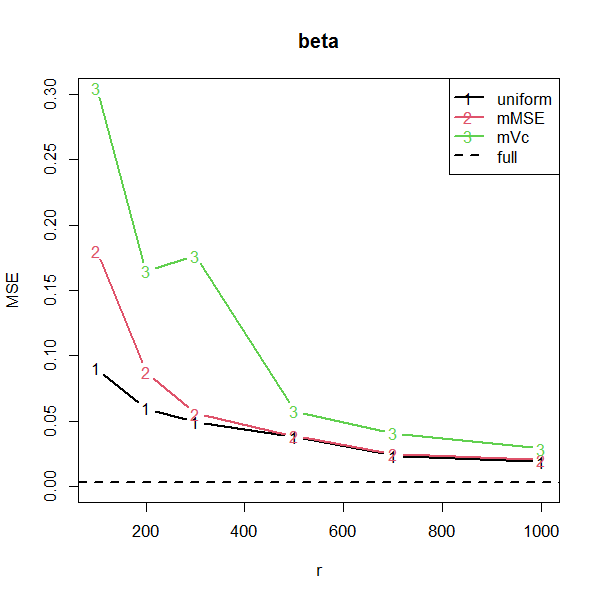
\includegraphics[width = .6\textwidth]{beta.png}
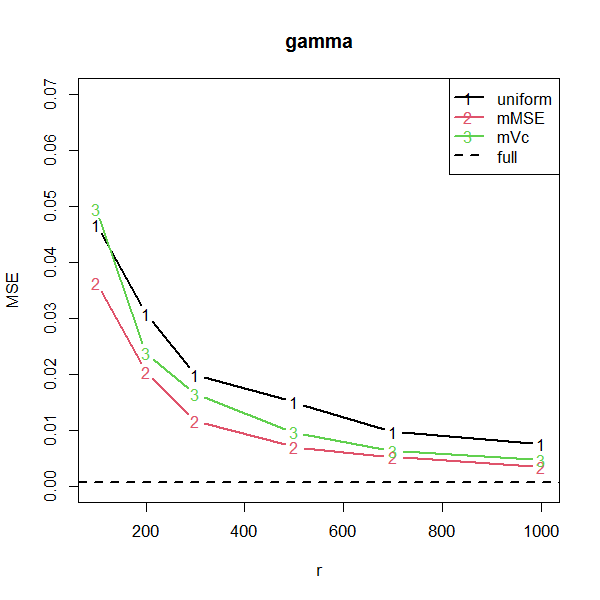
\includegraphics[width = .6\textwidth]{gamma.png}
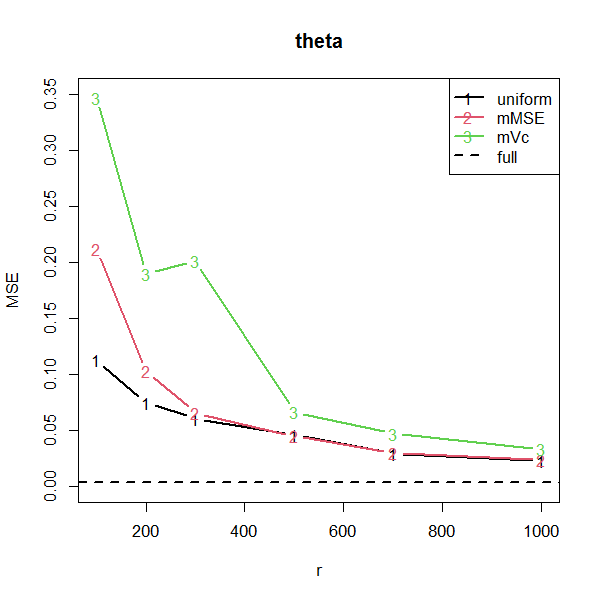
\includegraphics[width = .6\textwidth]{theta.png}
\\
It seems that the gradient and hessian (numerically evaluated) is not stable, and the variations for evaluating gradient and hessian are larger than the variation for uniform subsampling, especially for $\boldsymbol{\beta}$. ($\boldsymbol{\gamma}$ is always better than $\boldsymbol{\beta}$, in the limited simulations) 
















 












	
	
	
	
	
	
\end{document}